\documentclass{article}
\usepackage[letterpaper, margin=1in]{geometry}
\usepackage[utf8]{inputenc}
\usepackage{amsmath}
\usepackage{amssymb}
\usepackage{verbatim}
\usepackage{graphicx}
\graphicspath{ {Images/} }
\usepackage{pdfpages}
\usepackage{subcaption}
%\usepackage{physics} % For abs
\usepackage{wrapfig}

\usepackage[english]{babel}
\usepackage[backend=biber,style=ieee,sorting=ynt]{biblatex}
\addbibresource{Darve.bib}

\title{Exploring Hierarchical Layers in Deep Neural Networks \\
	\large Project Category: Computer Vision \\ 
	CS230 Project Proposal\\
	}
\author{Brian Jackson (bjack205)}
\date{January 2018}

\begin{document}
	\maketitle
	
	\section{Overview}
	Modern neural networks generally consist of two types of layers: fully-connected or convolutional. State-of-the-art object detectors such as YOLO \cite{Redmon2015,Redmon2016}, Fast R-CNN \cite{Girshick2015}, and SSD \cite{Liu2016} use deep neural networks with many convolutional layers. However, the increased performance of these systems has often come at significant computational expense. Fully-connected layers, in particular, require enormous amounts of memory and computation time. I propose to investigate the use of hierarchical layers to both reduce computational expense and potentially improve performance, in addition to applying some pruning and compression methods already implemented in previous papers \cite{Novikov2015,V.Oseledets2011,Han2015}. 
	
	\section{Methodology}
	\subsection{Model}
	I will focus this project on improving YOLO v2 \cite{Redmon2016}, since this neural network is one of the current state-of-the-art real-time object detection systems and also uses fully-connected layers at the end of a set of convolutional layers. Replacing these fully-connected layers with hierarchical layers will be the main focus of my project.
	
	\subsection{Dataset}
	
	I will be testing my algorithms on the KITTI data set \cite{KITTIDataset} and using the authors' vision dataset and benchmarking tools \cite{KITTIVision}. This dataset captures camera data from a car driving around urban and rural areas in a German town. I will be using the 2D object recognition dataset.
	
	\begin{wrapfigure}{O}{0pt}
		\centering
		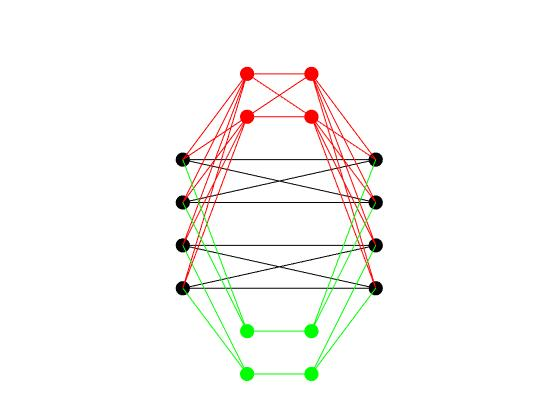
\includegraphics[width=0.5\textwidth]{HNN}
		\caption{Sample of proposed hierarchical layers.}
		\label{fig:hnn}
	\end{wrapfigure}
	
	\subsection{Experimentation}
	After training YOLO v2 on the dataset I will start by compressing the network using pruning and other compression techniques and evaluate changes in training and test speed and memory usage. The purpose of this will be to evaluate these methods on a ``real'' dataset that accurately portrays the types of images seen by autonomous vehicles. I expect to see decreases in computational requirements with negligible drops in mAP and other performance benchmarks provided by the dataset. I will then start replacing the fully-connected layers with hierarchical layers. Hierarchical layers maintain global connectivity while significantly reducing the number of edges. This is accomplished by grouping sets of neurons to a reduced number of neurons in the next layer. After a repeating this several times, these are expanded in a symmetric fashion back to the original shape (see Figure \ref{fig:hnn}) This will be the most challenging part of the project since it is a novel approach to neural networks and, to my knowledge, has never been applied to the task of object detection. I expect these layers will perform better than fully-connected layers at simultaneously combining lower-level details with high-level features, which should result in better detection accuracy while also decreasing computational requirements. 
	
	\subsection{Evaluation}
	As mentioned in the previous section, performance will be measured by evaluating the changes in object detection accuracy (both localization and classification) and computational requirements. I will show how specific changes affecting these criteria.
	
	\section{Conclusion}
	I propose to investigate methods of compressing the YOLO v2 framework and evaluate its performance on a real-world dataset for autonomous driving. I also will investigate the use of novel layer topologies that may offer new benefits to the field of deep learning and object recognition, in particular. 
	
	\section*{Acknowledgements}
	Professor Eric Darve in the Stanford Mechanical Engineering department has demonstrated that hierarchical layers show much promise and will be advising me on this project.
	 
	
	\printbibliography
	
\end{document}
